\documentclass[10pt,usenames,dvipsnames]{beamer}
\usepackage[english]{babel}
\usepackage{euler}

\usetheme{boxes}
%\useoutertheme{essential}
\usecolortheme{seagull}
\usefonttheme{professionalfonts}
\usefonttheme{structurebold}
\setbeamertemplate{navigation symbols}{}
\setbeamertemplate{frametitle}
{
	\begin{centering}
		\vspace{1.5em}
		\LARGE
    \insertframetitle
    \par
    %\vspace{0.5em}
  \end{centering}
}
\setbeamerfont{title}{size=\huge}
\setbeamerfont{subtitle}{size=\Large}
\renewcommand{\thefootnote}{\textsf{\fnsymbol{footnote}}}

% footnote refs per frame
\AtBeginEnvironment{frame}{\setcounter{footnote}{0}}

\usepackage[no-math]{fontspec}

\usepackage{tikz}
\usepackage{listings}
\usepackage{relsize}
\usepackage{array}
\usepackage{booktabs}
\usepackage{ragged2e}
\usepackage{varwidth}
\usepackage{multicol}
\usepackage{amsmath}

\makeatletter
\newlength{\negph@width}%
\newcommand{\negphantom}[1]{%
\settowidth{\negph@width}{#1}%
\hspace{-\negph@width}%
}
\makeatother

\newcommand{\aligntext}[2]{%
#2\negphantom{#2}\hphantom{#1}%
}

\setmainfont{texgyretermes}[
  Path=../fonts/,
  Extension=.otf,
  UprightFont=*-regular,
  BoldFont=*-bold,
  ItalicFont=*-italic,
  BoldItalicFont=*-bolditalic]
\setsansfont{texgyreheros}[
  Path=../fonts/,
  Extension=.otf,
  UprightFont=*-regular,
  BoldFont=*-bold,
  ItalicFont=*-italic,
  BoldItalicFont=*-bolditalic]
\setmonofont{RecMono-Casual}[
  Path=../fonts/,
  Extension=.ttf,
  BoldFont=*Bold,
  ItalicFont=*Italic,
  BoldItalicFont=*BoldItalic]

\usetikzlibrary{arrows}
\usetikzlibrary{backgrounds}
\usetikzlibrary{chains}
\usetikzlibrary{fit}
\usetikzlibrary{positioning}
\usetikzlibrary{scopes}
\usetikzlibrary{trees}
\usetikzlibrary{automata}
\usetikzlibrary{positioning}
\usetikzlibrary{shapes.multipart}

\lstset{basicstyle=\ttfamily}
\newcommand{\txtinput}[2][\ttfamily]{\lstinputlisting[language=none,basicstyle=#1]{#2}}
\newcommand{\txtinline}[2][\ttfamily]{\lstinline[language=none,basicstyle=#1]!#2!}
\newcommand{\cinput}[2][\ttfamily]{\lstinputlisting[language=C,basicstyle=#1]{#2}}
\newcommand{\cinline}[2][\ttfamily]{\lstinline[language=C,basicstyle=#1]!#2!}
\newcommand{\cppinput}[2][\ttfamily]{\lstinputlisting[language=C++,basicstyle=#1]{#2}}
\newcommand{\cppinline}[2][\ttfamily]{\lstinline[language=C++,basicstyle=#1]!#2!}
\newcommand{\llvminput}[2][\ttfamily]{\lstinputlisting[language=LLVM,basicstyle=#1]{#2}}
\newcommand{\llvminline}[2][\ttfamily]{\lstinline[language=LLVM,basicstyle=#1]!#2!}
\newcommand{\asminput}[2][\ttfamily]{\lstinputlisting[language=x86gas,basicstyle=#1]{#2}}
\newcommand{\asminline}[2][\ttfamily]{\lstinline[language=x86gas,basicstyle=#1]!#2!}
\lstdefinelanguage{LLVM}%
  {morekeywords={define,declare,global,constant,internal,external,private,%
      linkonce,linkonce_odr,weak,weak_odr,appending,common,extern_weak,%
      thread_local,dllimport,dllexport,hidden,protected,default,except,deplibs,%
      volatile,fastcc,coldcc,cc,ccc,x86_stdcallcc,x86_fastcallcc,ptx_kernel,%
      ptx_device,signext,zeroext,inreg,sret,nounwind,noreturn,nocapture,byval,%
      nest,readnone,readonly,noalias,uwtable,inlinehint,noinline,alwaysinline,%
      optsize,ssp,sspreq,noredzone,noimplicitfloat,naked,alignstack,module,asm,%
      align,tail,to,addrspace,section,alias,sideeffect,c,gc,target,datalayout,%
      triple,blockaddress},%
  morekeywords=[2]{add,fadd,sub,fsub,mul,fmul,sdiv,udiv,fdiv,srem,urem,frem,%
     and,or,xor,icmp,fcmp,eq,ne,ugt,uge,ult,ule,sgt,sge,slt,sle,oeq,ogt,oge,%
     olt,ole,one,ord,ueq,ugt,uge,ult,ule,une,uno,nuw,nsw,exact,inbounds,phi,%
     call,select,shl,lshr,ashr,va_arg,trunc,zext,sext,fptrunc,fpext,fptoui,%
     fptosi,uitofp,sitofp,ptrtoint,inttoptr,bitcast,ret,br,indirectbr,switch,%
     invoke,unwind,unreachable,malloc,alloca,free,load,store,getelementptr,%
     extractelement,insertelement,shufflevector,extractvalue,insertvalue},%
  sensitive=t,%
  morestring=[b]",%
  morecomment=[l];%
  }[keywords,comments,strings]
\lstdefinelanguage{x86gas}%
  {morekeywords={%
.abort, .ABORT, .align, .ascii, .asciz, .balign, .bss, .bundle, .byte, .cfi, %
.comm, .cstring, .data, .def, .desc, .dim, .double, .eject, .else, .elseif, %
.end, .endef, .endfunc, .endif, .equ, .equiv, .eqv, .err, .error, .exitm, %
.extern, .fail, .file, .fill, .float, .func, .global, .globl, .gnu, .hidden, %
.hword, .ident, .if, .incbin, .include, .int, .internal, .irp, .irpc, .lcomm, %
.lflags, .line, .ln, .linkonce, .list, .loc, .local, .long, .macro, .mri, %
.noaltmacro, .nolist, .octa, .offset, .org, .p2align, .popsection, .previous, %
.print, .protected, .psize, .purgem, .pushsection, .quad, .rept, .sbttl, .scl, %
.section, .set, .short, .single, .size, .skip, .sleb128, .space, .stabd, %
.stabn, .stabs, .string, .struct, .subsection, .symver, .tag, .text, .title, %
.type, .uleb128, .val, .version, .vtable, 	.vtable_entry, 	.vtable_inherit, %
.warning, .weak, .weakref, .word, .zero
},%
  morekeywords=[2]{%
aaa, adcb, adcl, add, addb, addl, addps, addw, addq, adds, addss, addsd, and, %
andb, andw, andl, andq, bswap, call, callq, cld, cltd, cltq, cmova, cmovae, %
cmovb, cmovbe, cmovg, cmovge, cmovl, cmovle, cmovna, cmovnae, cmovnb, cmovnbe, %
cmovne, cmovng, cmovnge, cmovnl, cmovnle, cmovns, cmovnz, cmovs, cmovz, cmp, %
cmpb, cmpeqps, cmpl, cmpq, cmpsl, cmpxchg, cpuid, cqto, cvtps2dq, cvtdq2ps, %
cvtsd2ss, cvtsi2s, cvtsi2ss, cvtsi2ssq, cvtsi2sd, cvtsi2sdq, cvtss2sd, cvttsd, %
cvttsd2si, cvttsd2siq, cvtts, cvttss, cvttss2si, cvttss2siq, das, dec, decb, %
decw, decl, decq, divw, divl, divq, divs, divss, divsd, fabs, fadd, fbld, %
fbstp, fchs, fcmovb, fcomi, fcoms, fcos, fdivp, fdivr, fdivrp, fidivs, filds, %
fimul, finit, fists, fld1, fldcw, fldl, fldl2t, fldl2e, fldlenv, fldlcw, %
fldlg2, fldln2, fldpi, flds, fldz, fmul, fmulp, fprem1, frame, frndint, %
frstor, fsave, fsin, fsincos, fsqrt, fst, fstcw, fstl, fstps, fsts, fstsw, %
fstenv, fstpl, fstsw, fsubr, fxch, fyl2x, idivl, idivq, imul, imulb, imull, %
imulw, imulq, inc, incb, incw, incl, incq, int, ja, jb, jc, jcxz, je, jg, jge, %
jl, jmp, jne, jns, jnz, jo, jp, js, jz, lea, leab, leave, leawl, leaq, leal, %
lodsb, lodsl, loop, maxps, maxs, maxss, maxsd, mins, minss, minssd, mov, %
movabsq, movapd, movaps, movqps, movb, movdqa, movdqu, movl, movlpd, movq, %
movupd, movups, movsb, movsbw, movsbl, movsbq, movsd, movsl, movslq, movsw, %
movswl, movswq, movsx, movss, movsd, movw, movz, movzbw, movzbl, movzbq, %
movzwl, movzwq, movzx, msg, mull, mulpd, muls, mulss, mulsd, mulq, neg, negb, %
negw, negl, negq, nop, not, notb, notw, notl, notq, or, orb, orw, orl, orq, %
paddd, pcmpeqw, pop, popfl, popl, popq, popw, push, pushfl, pushl, pushq, %
pushw, rep, repe, repne, ret, retq, rspreg, sahf, sal, salb, salw, sall, salq, %
sar, sarb, sarw, sarl, sarq, sbbb, sbbl, shr, shrb, shrw, shrl, shrq, sqrtps, %
sqrts, sqrtss, sqrtsd, std, stosb, sub, subb, subl, subq, subw, subs, subss, %
subsd, syscall, test, testb, testq, ucomis, ucomisd, ucomiss, xchg, xor, xorb, %
xorps, xorw, xorl, xorq, vxorpd, vaddsd},%
  sensitive=t,%
  morestring=[b]",%
  morecomment=[l]\#%
  }[keywords,comments,strings]
\lstdefinelanguage{none}{
  identifierstyle=
}
  
% Create Color definition From Template: 
% #1 template name, 
% #2 foreground color name
% #3 background color name
\newcommand{\ccft}[3]{
\usebeamercolor{#1}
\definecolor{#2}{named}{fg}
\definecolor{#3}{named}{bg}
}
\ccft{palette primary}{ThemePriFg}{ThemePriBg}
\ccft{palette secondary}{ThemeSecFg}{ThemeSecBg}
\ccft{palette tertiary}{ThemeTerFg}{ThemeTerBg}
\ccft{palette quaternary}{ThemeQuaFg}{ThemeQuaBg}



\author{Daniele Cattaneo}
\institute{Politecnico di Milano}
\date{\DATE}
\title{The LLVM compiler framework}
\subtitle{Writing a pass: Quick Start}
\newcommand{\customdata}{Daniele Cattaneo <stefano.cherubin@polimi.it>}

\AtBeginSection[]
{
\begin{frame}{Contents}
\tableofcontents[currentsection]
\end{frame}
}


\begin{document}

\begin{frame}
\maketitle
\begin{center}
\itshape\scriptsize
These slides were originally written by
Stefano Cherubin for the
``Code Transformation and Optimization'' course.
\end{center}
\end{frame}

% !TEX root = main.tex

\section{Introduction}


\begin{frame}{Understanding LLVM}
	\begin{center}
	\huge{
		LLVM is \textbf{not} a compiler.\\
		\pause
		\vfill
		LLVM is a\\\textbf{collection of components}\\
		which is \textbf{useful}\\to build a compiler.
	}
	\end{center}
\end{frame}


\begin{frame}{Getting LLVM}
\begin{itemize}
	\item ``old'' git mirrors
		\begin{itemize}
			\item only llvm repo (subprojects in separated repos, can be added later)
			\item \texttt{git clone -b release\_90 --single-branch git@github.com:llvm-mirror/llvm.git}
		\end{itemize}
	\vfill
	\item ``new'' git monorepo
		\begin{itemize}
			\item all in one repo (llvm + major subprojects)
			\item \texttt{git clone -b release/9.x --single-branch git@github.com:llvm/llvm-project.git}
		\end{itemize}
\end{itemize}
\end{frame}


\begin{frame}{What LLVM is made of}
\begin{itemize}
	\item C++ libraries
		\begin{itemize}
			\item \texttt{src/include/llvm/...}
			\item \texttt{src/lib/...}
		\end{itemize}
		\vfill
	\item small application (tools)
		\begin{itemize}
			\item \texttt{src/tools/...}
			\item \texttt{src/utils/...}
		\end{itemize}
\end{itemize}
\vfill
You can find binaries of them in the installation directory under \texttt{root/bin/...}
\end{frame}


\begin{frame}{clang}
\begin{itemize}
	\item \texttt{clang} is a compiler based on LLVM
	\item It compiles all major C-like languages
	\vfill
	\item It is part of the git monorepo
	\item It can be added as a tool in the LLVM framework but must be manually cloned in the tool directory
	\begin{enumerate}
		\item \texttt{cd src/tools}
		\item \texttt{git clone http://llvm.org/git/clang} (git mirror version)
	\end{enumerate}
	\vfill
	\item You can easily see on a production quality compiler the impact of changes you made on your local copy of LLVM
\end{itemize}
\end{frame}


\begin{frame}{Commands}
	\begin{description}[llvm-dwarfdump]
		\item[llvm-as] LLVM assembler
		\item[llvm-dis] LLVM disassembler
		\item[opt] LLVM optimizer
		\item[llc] LLVM static compiler
		\item[lli] directly execute programs from LLVM bitcode
		\item[llvm-link] LLVM bitcode linker
		\item[llvm-mca] LLVM machine code analyzer
		\item[llvm-nm] list LLVM bitcode and object file's symbol table
		\item[llvm-stress] generate random .ll files
		\item[llvm-config] prints out install configuration parameters
		\item[llvm-dwarfdump] print contents of DWARF sections
	\end{description}
	\vfill
	For a complete reference, see the LLVM command guide\footnote{\url{http://llvm.org/docs/CommandGuide/index.html}}
\end{frame}



% !TEX root = main.tex

\section{LLVM framework quick start}


\begin{frame}{Simulating a LLVM driver manually}
%	\noindent\hspace{-1.2cm}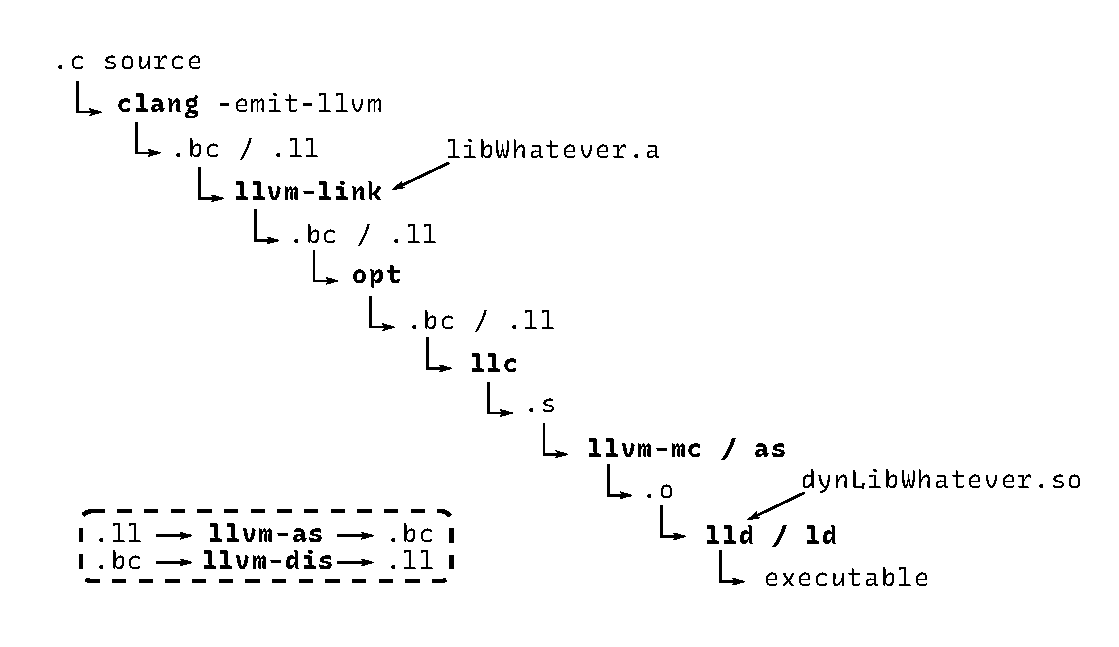
\includegraphics[width=13cm]{img/toolchain}
\begin{center}
\begin{tikzpicture}[yscale=0.55,xscale=0.6]
\node[anchor=west] (step0) at (0,0) {\texttt{.c} source};
\node[anchor=west] (step1) at (1,-1) {\texttt{\textbf{clang} -emit-llvm}};
\node[anchor=west] (step2) at (2,-2) {\texttt{.bc}/\texttt{.ll}};
\node[anchor=west] (step3) at (3,-3) {\texttt{\textbf{llvm-link}}};
\node[anchor=west] (step4) at (4,-4) {\texttt{.bc}/\texttt{.ll}};
\node[anchor=west] (step5) at (5,-5) {\texttt{\textbf{opt}}};
\node[anchor=west] (step6) at (6,-6) {\texttt{.bc}/\texttt{.ll}};
\node[anchor=west] (step7) at (7,-7) {\texttt{\textbf{llc}}};
\node[anchor=west] (step8) at (8,-8) {\texttt{.s}};
\node[anchor=west] (step9) at (9,-9) {\textbf{\texttt{llvm-mc}/\texttt{as}}};
\node[anchor=west] (step10) at (10,-10) {\texttt{.o}};
\node[anchor=west] (step11) at (11,-11) {\textbf{\texttt{lld}/\texttt{ld}}};
\node[anchor=west] (step12) at (12,-12) {executable};
\foreach \i in {0,...,11}{
  \draw[->] ($(\i+0.5,-\i-0.5)$) |- ($(\i+1,-\i-1)$);
}
%\node[anchor=south west, above right=0.2ex and 1.5em of step3.north east] (note0) {\texttt{libWhatever.a}};
%\draw[->] ($(note0.south west)+(0.5em,0.5ex)$) -- (step3.east);
\node[anchor=south west, above right=0.2ex and -1em of step11.north east] (note1) {\texttt{libWhatever.a}};
\draw[->] ($(note1.south west)+(0.5em,0.5ex)$) -- ($(step11.north)+(-0.5em,0)$);
\node[anchor=south west,draw,dashed,very thick,rounded corners=5pt,align=center] at (0,-12) 
  {\texttt{.ll} $\rightarrow$ \texttt{\textbf{llvm-as}} $\rightarrow$ \texttt{.bc}\\
  \texttt{.bc} $\rightarrow$ \texttt{\textbf{llvm-dis}} $\rightarrow$ \texttt{.ll}};
\end{tikzpicture}
\end{center}
\end{frame}


\begin{frame}{Writing a LLVM pass}
	There are a lot of tutorials available:
	\vfill
	\begin{itemize}
		\item Official developer guide\\ \href{https://llvm.org/docs/WritingAnLLVMNewPMPass.html}{\url{https://llvm.org/docs/WritingAnLLVMNewPMPass.html}}
		\vfill
		\item Out-of-source pass\\ \href{https://github.com/quarkslab/llvm-dev-meeting-tutorial-2015}{\url{github.com/quarkslab/llvm-dev-meeting-tutorial-2015}}
	\end{itemize}
	\vfill
	We will follow the first one, with a few adjustments.
\end{frame}


\begin{frame}{Building LLVM}
\begin{center}
To test your pass you need a \alert{Debug+Assertions} build of LLVM.\\
\bigskip
This build needs to be \alert{kept separated} from normal Release builds (it's very slow!)\\
\bigskip
The best way to get such a LLVM build is to \alert{make it yourself}!
\end{center}
\end{frame}


\begin{frame}{Building LLVM}
\begin{itemize}
\item Detailed instructions: \url{https://llvm.org/docs/GettingStarted.html}
\end{itemize}
\bigskip
\begin{description}
\item[Problem 1] With the \alert{default options}, a finished build takes\\\alert{25 GB of disk space}
\item[Problem 2] A standard build with the GNU toolchain uses \alert{a lot of RAM} ($\approx$16 GB or more with a modern 4 core CPU!) especially when linking
\end{description}
\bigskip
We need to customize the build process a bit...
\end{frame}


\begin{frame}{Building LLVM}
\begin{itemize}
\item The build flags I like to use:\\
\smallskip\texttt{\small-GNinja \\
-DCMAKE\_BUILD\_TYPE=Debug\\
-DLLVM\_ENABLE\_PROJECTS='clang;compiler-rt' \\
-DLLVM\_INSTALL\_UTILS=ON \\
\textbf{-DLLVM\_BUILD\_LLVM\_DYLIB=ON \\
-DLLVM\_LINK\_LLVM\_DYLIB=ON} \\
-DLLVM\_OPTIMIZED\_TABLEGEN=ON \\
-DLLVM\_INCLUDE\_EXAMPLES=OFF \\
-DCMAKE\_INSTALL\_PREFIX=/opt/llvm-18-d \\
\textbf{-DLLVM\_USE\_LINKER=lld \\
-DCMAKE\_C\_COMPILER=clang-18 \\
-DCMAKE\_CXX\_COMPILER=clang++-18} \\
}
\item Building with LLVM itself solves the RAM usage problem!
	\begin{itemize}
	\item Not required on macOS or *BSD: they already ship LLVM as default
	\end{itemize}
\item Using \alert{shared libraries} drops the disk usage to \alert{10 GB}.\\
{\footnotesize The build products alone will still take 20 GB of disk space...}
\end{itemize}
\end{frame}


\begin{frame}{Last notes on building}
You can add other projects to the LLVM build by modifying the value of the \texttt{LLVM\_ENABLE\_PROJECTS} flag\\
\bigskip
Good practice: \alert{always include clang}
\begin{itemize}
	\item You can easily see on a production quality compiler the impact of changes you made on your local copy of LLVM
\end{itemize}
\bigskip
To install cutting-edge release LLVM if your Linux distribution does not provide it:\\
\begin{itemize}
	\item \url{https://apt.llvm.org}
\end{itemize}
\end{frame}


\begin{frame}{Testing}
LLVM has an internal testing infrastructure\footnote{\url{http://llvm.org/docs/TestingGuide.html}}.
Please use it.
\\
\begin{description}
	\item[llvm-lit] LLVM Integrated Tester
\end{description}
\begin{enumerate}
	\item Forge a proper LLVM-IR input file (.ll) for your test case
	\item Instrument it with \texttt{lit} script comments
	\item Run \texttt{lit} on your test
		\begin{itemize}
			\item \texttt{llvm-lit ~/llvm/test/myTests/singleTest.ll}\\ run a single test
			\item \texttt{llvm-lit ~/llvm/test/myTests}\\ run the test suite (folder)
		\end{itemize}
	\item Run \texttt{lit} on the LLVM test suite (regression testing)
\end{enumerate}
\vfill
To submit a bug report to LLVM developers you will be asked to write a \texttt{lit} test case that highlights the bug.
\end{frame}



\end{document}
